\documentclass[11pt]{article}
\usepackage{acl2014}
\usepackage{times}
\usepackage{url}
\usepackage{latexsym}
\usepackage[utf8]{inputenc}
\usepackage{color}
\usepackage{xspace}
\usepackage{url}

\usepackage{amsmath}
%%\usepackage{color}
\usepackage{amsfonts}
\usepackage{amssymb}
\usepackage{graphicx}
\usepackage{multirow}


\def \xxx#1{\textbf{\textcolor{red}{xxx: #1}}}
\def \todo#1{\textbf{\textcolor{red}{todo: #1}}}
\def\equo#1{``#1''}

\def\Tref#1{Table~\ref{#1}}
\def\Fref#1{Figure~\ref{#1}}
\def\Sref#1{Section~\ref{#1}}
\newcommand{\out}[1]{\textcolor[rgb]{0.8,0.8,0.8}{\textbf{#1}}}
\newcommand{\ml}[1]{\textcolor{red}{\raisebox{.2ex}{\tiny ML:~}#1}}
%\def\footurl#1{\footnote{\url{#1}}}

%\usepackage[left=2cm,right=2cm,top=2cm,bottom=2cm]{geometry}

\title{Parmesan: Meteor without Paraphrases with Paraphrased References}

\author{Petra Barančíková \\
  Institute of Formal and Applied Linguistics \\
  Charles University in Prague, Faculty of Mathematics and Physics\\
  Malostranské náměstí 25, Prague, Czech Republic \\
  {\tt barancikova@ufal.mff.cuni.cz} \\}
%Hackers not welcome here!
\date{}
%
%This paper describes Parmesan, our submission to the 2014 Workshop on Statistical Machine Translation (WMT) metrics task for evaluation English-to-Czech translation. 
%We show that the Czech Meteor Paraphrase tables are so noisy that they actually can harm the performance of the metric. However, they can be very useful after extensive filtering in targeted paraphrasing of Czech reference sentences prior to the evaluation.
%Parmesan first performs targeted paraphrasing of reference sentences, then it computes the Meteor score using only the exact match on these new reference sentences. It shows significantly higher correlation with human judgment than Meteor on the WMT12 and WMT13 data. However, this result was not confirmed by this year's data.

\begin{document}

\maketitle
\begin{abstract}
This thesis is concentrated on improving an accuracy of machine translation
to Czech language using targeted paraphrasing. We develop system that creates
new synthetic reference that are closer in wording to a corresponding machine
translations. Using these new reference sentences makes evaluation using traditional
metrics is more reliable as they lack of paraphrase support and have no sympathy
for a free word order.

We believe that after implementation, the system for generating new syntetic
references will be very beneficial not only for MT evaluation, but mainly
inside MT systems for improved tuning and development of the systems. This way,
it will directly influence the quality of machine translation itself.

%Trade-off between simplicity and quality of MT metric!!
\end{abstract}

\section{Introduction}
Since the very first appearance of machine translation (MT) systems, a necessity
for their objective evaluation and comparison arose. The traditional human evaluation 
while being the most reliable has serious drawbacks -- it is time-consuming and expensive.
.%, although there were recently successful attempts to overcome this problem using crowdsourcing techniques. [\markcite{{\it Callison-Burch}, 2009]} and [\markcite{{\it Bentivogli et al.}, 2011]} demonstrate that the average score of high number of non-expert low-paid annotators shows high agreement with gold standards provided by expert annotators in various natural language processing (NLP) tasks including machine translation evaluation.

However, the main problem of human evaluation is that it is highly dependent on the 
person annotating and there is generally very low agreement between several human
annotators. %footnote - example, only blah blah correlation during \cite{wmt12}.
Moreover, it is practically impossible to repeat the evaluation with the same
results (TODO: nejaka citace).
%[Bojar - kniha] %nizka shoda pro cestinu?!! Ani ne kniha, ale spis wmt13, co 14?, 
% kde to byla nejak hrozive nizka shoda..

Due to being slow and unreproducible, it is impossible to use human evaluation
for tuning and development of MT systems. Well-performing automatic MT evaluation
metrics are essential precisely for these tasks.

The first metric correlating well with human judgment was BLEU \cite{bleu} and
it still remains the most common metric for MT evaluation, even though other,
better-performing metrics exist. \cite{wmt13-metrics} %sem mozna uz wmt14?

BLEU is computed from the number of phrase overlaps between the translated
% sem by se hodil asi opravdovej vzorecek misto jen zminy. nebo jen odkaz
% do sekce Automatic metrics?? asi tak
sentence (hypothesis) and the corresponding reference sentences, i.e., translations
made by a human translator. Its main advantage is its simplicity and language independence. 
However, the standard practice is using only one reference sentence and BLEU then tends 
to perform badly. As there are many translations of 
a single sentence, even a perfectly correct machine translation might get a low score 
due different wording and disregarding synonymous expressions (see \Fref{example_of_BLEU_malfunction}). 
This is especially valid for morphologically rich languages with free word order like 
the Czech language. \cite{bojar-tackling-sparse-data}

\begin{figure*}[htb]
\begin{center}
\begin{tabular}{ll}
 Original sentence &  \begin{tabular}{l}
  	\textit{Banks are testing payment by mobile telephone} \\
	\end{tabular}  \\
 \hline
 
 MT output & \begin{tabular}{llllll}
 			\textit{Banky} & \textit{zkou\v sej\'i} & \textit{platbu} & \textit{pomoc\'i} & \textit{mobiln\'iho} & \textit{telefonu} \\
 			Banks & are testing & payment & with help & mobile & phone \\
			\end{tabular} \\
 & \begin{tabular}{l}
  	Banks are testing payment by mobile phone \\
	\end{tabular} \\

% MT output & \textit{Banky zkou\v sej\'i platbu pomoc\'i mobiln\'iho telefonu} \\
% 					 & Banks testing payment help mobile phone \\
% 					 & Banks are testing payment by mobile telephone \\
 \hline
 Reference sentence & \begin{tabular}{llll}
 			\textit{Banky} & \textit{testuj\'i} & \textit{placen\'i} & \textit{mobilem} \\
 			Banks & are testing & paying & by mobile phone \\
			\end{tabular} \\
 &  \begin{tabular}{l}
  	Banks are testing paying by mobile phone \\
	\end{tabular}
 
\end{tabular}
\caption{Example from WMT12 - Even though the translation is grammatically 
correct and the meaning of both sentences is very similar, it doesn't contribute 
to the BLEU score. There is only one unigram overlapping.}
\end{center}
\label{example_of_BLEU_malfunction}
\end{figure*}

We aim to achieve higher accuracy of MT evaluation by targeted paraphrasing 
of reference sentences, i.e. creating a new synthetic reference sentence that 
is still correct and keeps the meaning of the original sentence, but at the 
same time it is closer in wording to the MT output. 


\section{Related Work}
There are two attitudes towards solving the problem - one is to change the automatic
metric itself to be tolerant to other sentence representation and the other one is to 
preprocess automatically the reference sentence to new synthetic reference that is closer 
in wording to the original reference sentence and keeps its meaning and grammatical correctness.

\subsection{New synthetic references}
Targeted paraphrasing for MT evaluation is introduced in~\newcite{kauchak}. They 
improve the accuracy of~MT evaluation of Chinese-to-English translation by targeted 
paraphrasing.

Having a hypothesis $ H = h_1,...,h_n $ and its corresponding reference translation 
$ R =r_1, ...,r_m $, they select a~set of~candidates 
$ C = \lbrace \langle r_i,h_j \rangle  \vert r_i \in R \setminus H, h_j \in H \setminus R \rbrace $. 
 
$ C $~is reduced to pairs of words appearing in~the~same WordNet synset only. For every pair 
$  \langle r_i,h_j \rangle \in C $, $ h_j $ is evaluated in the context $ r_1,...,r_{i-1},\square,r_{i+1},...,r_m $
and if confirmed, the new reference sentence $ r_1,...,r_{i-1},h_j,r_{i+1},...,r_m $ is created.
This way, several reference sentences might be created, all with a single changed word with respect
to the original one.

%
%Targeted paraphrasing for MT evaluation is introduced in~\newcite{kauchak}. They 
%focus on lexical substitution in Chinese-to-English translations. 
%They select all pairs of words for which one word appears in a reference sentence,
%second word in a hypothesis (the MT output), but none of them in both. They keep 
%only pairs of synonymous words, i.e. words appearing in the same WordNet 
%\cite{wordnet} synset. Each such a pair of words was further contextually evaluated. 
%For every confirmed synonym, a new reference sentence is created by placing it to the
%reference sentence on the position of its synonym.
%

This solution is not quite possible to apply to the Czech language. As Czech belongs 
among~inflective languages with rich morphology, a Czech word has typically many forms 
and the correct form depends heavily on its context, e.g., cases of nouns depend on verb 
valency frames. Changing a single word may result into not grammatical sentence. Therefore, 
we do not attempt to~change a~single word in~a~reference sentence but we focus on~creating 
one single correct reference sentence.

%jeste zapojit \cite{Zhou:2006}

\subsection{Automatic Metrics}
BLEU (and other commonly used metrics - NIST \cite{nist}, TER \cite{ter} etc.) 
disregards synonymous phrases and word form variants. One way how to  alleviate this 
drawback is to include paraphrases to the evaluation metric (e.g. METEOR \cite{meteor}). 

But this often awards even sentences with paraphrases that are not grammatically correct. 
We take a different approach by transforming a reference translation into a sentence that 
is closer to the MT output and keeps its original meaning and correctness.

There are several metrics that include paraphrase support, however only the Meteor metric
is available for Czech language too.%TODO: preformulovat

\subsubsection{Meteor}
The Meteor metric \cite{meteor-wmt:2011} has shown high correlation with human 
judgement since its appearance. It outperforms traditional metrics like BLEU \cite{bleu} 
or NIST \cite{nist} as it explicitly addresses their weaknesses -- it takes into account 
recall, distinguishes between functional and content words, allows language-specific 
tuning of parameters and many others.

Another important advantage of Meteor is that it supports not only exact word matches 
between a hypothesis and its corresponding reference sentence, but also matches on the 
level of stems, synonyms and paraphrases. The Meteor Paraphrase tables \cite{meteor-tables} 
were created automatically using the \textit{pivot} method \cite{pivoting} for~six languages 
(TODO: which ones).

The basic setting of Meteor for evaluation of~Czech sentences offers two levels of matches -- 
exact and paraphrase. Further (TODO: odkaz), we show the impact of the quality of paraphrases 
on the performance of Meteor. We demonstrate that the Czech Meteor Paraphrase tables are full 
of noise and their addition to the metric worsens its correlation with human judgement. 

However, they can be very useful (after extensive filtering) in creating new reference sentences 
by~targeted paraphrasing. 
%This metric is basically an adaptation of~Meteor to~higher quality paraphrases.
We show that the Czech Meteor Paraphrase tables are so noisy that they actually can harm 
the performance of the metric. However, they can be very useful after extensive filtering 
in targeted paraphrasing of Czech reference sentences prior to the evaluation.
Parmesan first performs targeted paraphrasing of reference sentences, then it computes 
the Meteor score using only the exact match on~these new reference sentences. It shows 
significantly higher correlation with human judgment than Meteor on the WMT12 and WMT13 data. 
%Using the reduced and modified Czech Meteor Paraphrase tables and WordNet, Parmesan first creates 
%for every hypothesis a new reference sentence that is closer in~wording to the hypothesis, but 
%keeps its original meaning and correctness. Then it computes the Meteor score using only the 
%exact match on~these new reference sentences.

\section{Data}
\subsection{Text Data}
We perform our experiments on data sets from the English-to-Czech translation 
task of WMT12 \cite{wmt12}, WMT13 \cite{wmt13} and WMT14 \cite{wmt14}. The data 
sets contain 13/14\footnote{We use only 12 of them because two of them (FDA.2878 
and online-G) have no human judgments.}/10 files with Czech outputs of MT systems.

In addition, each data set contains one file with corresponding reference sentences 
and one with original English source sentences. We perform morphological analysis 
and tagging of the hypotheses and the reference sentences using Morče \cite{morce:2007}.

The human judgment of hypotheses is available as a relative ranking of performance of 
five systems for~a~sentence. We calculated the score for every system by the “$ > $ others” 
method \cite{bojar-grains}, which was the WMT12 official system score. It is computed 
as $ \frac{wins}{wins+loses} $. We refer to this interpretation of human judgment as 
\textit{silver standard} to distinguish it from the official system scores, which were 
computed differently each year (here referred to as \textit{gold standard}).

\subsection{Sources of Paraphrases}
\label{meteori}
We make use of all existing sources of Czech paraphrases -- the Czech WordNet 1.9 PDT 
\cite{czech-wordnet}, the Meteor Paraphrase Tables \cite{meteor-tables} and Czech PPDB %TODO: cite 
, which recently became available.

The Czech WordNet 1.9 PDT is derived from the WordNet \cite{wordnet} by automatic translation 
followed by manual verification. It~contains rather high quality lemmatized paraphrases. However 
their amount is~insufficient for our purposes %(see\Tref{number_of_substitutions}).  
%It contains 13k pairs of synonymous lemmas and 
- only one paraphrase per four sentences on~average is found in~the data. % (see \Tref{number_of_substitutions}).  

On~the other hand, Czech Meteor Paraphrase tables are quite the opposite of Czech WordNet -- 
they are large in size, but contain a lot of noise as they are constructed automatically 
from parallel data via pivoting \cite{pivoting}. 

The noise was particularly high among the multiword paraphrases -- for example: \textit{svého názoru} 
(its opinion) and \textit{šermovat rukama a mlátit neviditelného} (to flail one's arms and to beat 
the invisible one) are selected as a paraphrase. In \ref{multiword_filtering}, we show that the amount 
of noise in the multi-word paraphrases is so high that no automatic filtering method we used outperforms 
omitting them completely. Therefore, we used the multiword paraphrases only in our first experiment (see
\Sref{lrec}.

Among one-word paraphrases the noise is sparser, but there are still pairs like \textit{1873} - 
\textit{pijavice} (a leech) or \textit{afgh\'{a}nci} (Afghans) - \textit{š\v{t}astně} (happily) 
identified as synonyms. However, the biggest problem is that most of synonymous pairs were just 
different word forms of the same lemma. We performed automatically filtering among the one-word
paraphrases in the Meteor table, the method are described in \Sref{filtering-section}.


%\begin{table}[tb]
%\begin{center}
%\scalebox{0.97}{
%\begin{tabular}{l|ccc}
%& WMT12 & WMT13 & WMT14\\
%\hline
%WordNet            & 0.26 & 0.22 & 0.24\\
%filtered Meteor    & 1.53 & 1.29 & 1.39\\
%together           & 1.59 & 1.34 & 1.44\\
%\end{tabular}}
%\caption{Average number of one-word paraphrases per sentence found in WordNet, 
%filtered Meteor tables and their union over all systems.}
%\label{number_of_substitutions}
%\end{center}
%\end{table}

\subsubsection{Filtering the Meteor Tables}
\label{filtering-section}
We try to remove the noise from the data with two different methods. The first
one is based on manual error analysis and it is applied to~one-word pairs only.
The second one is fully automatic and can be applied on all data, but its results 
are inconclusive. Therefore, we employ only the first method in the rest of our 
experiments.

\subsection{Error-analysis Based Filtering}
We manually examine sentences after paraphrasing using only Meteor tables. Based on
our observation, we perform the following operations on pairs of one-word paraphrases 
from the Meteor tables:

\begin{itemize}
\item morphological analysis using Morče \cite{morce:2007} and replacing of word forms with their lemmas; 
\item removing pairs of identical lemmas;
\item removing pairs with different part of speech;
\item removing pairs of unknown words (typically foreign words).
\end{itemize}

The last two rules have a single exception -- paraphrases consisting of numeral and 
corresponding digits, e.g., \textit{osmnáct} (eighteen) and \textit{18}.\footnote{
\textit{0smnáct} has the part of speech \textit{C}, which is designated for numerals, 
\textit{18} is marked with \textit{X} meaning it is an unknown word for the morphological
analyzer.} These paraphrases are very common in the data. 

This way we reduce more than 160 000 pairs of one word paraphrases to only 32 154
couples of lemmas. All examples of bad one-word paraphrases from Subsection \ref{meteori} 
are removed.



We attempt to reduce the noise in the Czech Meteor Paraphrase tables in the following way. We 
keep only pairs consisting of single words since we were not successful in reducing the noise
effectively for the multi-word paraphrases \cite{barancikova2014}. 

Using Morče, we first perform morphological analysis of all one-word pairs and replace 
the word forms with their lemmas.  We keep only pairs of different lemmas. Further, we
 dispose of pairs of words that differ in their parts of speech (POS) or~contain an 
unknown word (typically a~foreign word). 

In this way we have reduced 684k paraphrases in~the original Czech Meteor Paraphrase tables 
to~only 32k pairs of lemmas. We refer to~this table as~filtered Meteor.

\section{New synthetic references}
In this section, we present our methods of paraphrasing reference sentences. We started
with simple greedy substitution similar to \cite{kauchak}. Then we used machine translation
systems themselves to create new references.

\subsection{Simple greedy substitution}
\label{lrec}
We experiment with several algorithms for paraphrasing reference sentences. They differ
in the method for selecting potential paraphrase pairs and in the choice of paraphrases.

\subsubsection{Candidate Selection}
We select potential paraphrases using two different methods. The first one is a simple 
greedy search similar to~\newcite{kauchak}, the other one uses automatic word alignment 
for selecting corresponding segments of~the reference sentence and the hypothesis.

\begin{description}
\item[Simple Greedy Method]
%\subsubsection{Simple Greedy Method}
Let $ r_1,..., r_n $,$ w_1,...,w_m $ be the hypothesis and the reference sentence, 
respectively. We performed their tagging and extracted sets of lemmas $ W_{L} $, $ R_{L} $.  
Then, one-word paraphrase candidates are chosen as:
$$ C_{L} = \lbrace (r,w) | r \in R_{L} \smallsetminus W_{L} \wedge w \in W_{L}
\smallsetminus R_{L}  \rbrace $$

Multi-words candidates $ C_M $ are selected as the Cartesian product of all sequences
from the reference sentence and all sequences from the hypothesis. Maximum phrase length 
is seven words, because that is the length of~the longest paraphrases in the data. Formally:

\begin{gather*}
C_{M} = \lbrace (<r_i,..,r_{i+x}>, <w_j,...,w_{j+y}>) | \: 1 \leq i \leq n-x \: \wedge \\ 
 \: 1~\leq~j \leq m-y  \: \wedge \: 0 \leq x,y \leq 6 \: \wedge \: (x \neq 0 \vee y \neq 0) \rbrace 
\end{gather*}
\item[Word and Phrase Alignments]
%\subsubsection{Word and Phrase Alignments}
%Due to a noisy source of our paraphrases, we experiment with adding word alignment.
One possible way to make the algorithm more reliable is to restrict the application of 
paraphrases to words/phrases which are aligned to each other. We compute word alignment 
between the reference translation and MT system outputs using GIZA++ \cite{gizapp}.

However, if we used only our test data to create the alignment (13 x 3003 + 12 x 3000 
= 75039 sentence pairs), the alignment quality would be insufficient. In order to make the 
training data for word alignment larger, we take advantage of the fact that all outputs are 
translations of the same data and also add all pairs of system outputs to our data, creating 
over 1,000,000 \equo{artificial} sentence pairs. For example, the parallel data for WMT12 then 
looks as follows:

\begin{center}
\begin{tabular}{ll}
Source & Target \\
\hline
system 1 & system 2 \\
system 1 & system 3 \\
... & ...\\
system 1 & system 13 \\
system 1 & reference \\
system 2 & system 1 \\
system 2 & system 3 \\
... & ... \\
system 13 & reference \\
\end{tabular}
\end{center}

We also experiment with adding much larger synthetic parallel data created by
machine translation (note that we need Czech-Czech data) but there was no impact
on the quality of paraphrasing so we follow the outlined approach which requires
no additional data or processing.

The set of~one-word candidates $C_L$ is then simply the set of all word pairs such
that there exists an alignment link between them. The set $C_M$ is extracted
using phrase extraction for phrase-based MT, the standard consistency criterion
is~applied \cite{Och99improvedalignment}.
\end{description}

\subsubsection{Paraphrasing}
We reduce the set $ C_{L} $ to pairs appearing in our paraphrase tables in the 
following way. If a word appears in several synonymous pairs we give preference 
to those found in~WordNet or even better in the intersection of paraphrases from 
WordNet and filtered Meteor. Similarly, we filter $ C_{M} $ to pairs also contained 
in the multi-word Meteor tables.

We evaluate three different paraphrasing methods which differ in the order of
substitution.

\begin{description}
\item[One-word only] We proceed word by word from the beginning of the reference 
sentence to~its end. If a~lemma of~a~word appears as~the first member of~a~pair 
in reduced $ C_{L} $, it is replaced by~the word from hypothesis that has its lemma
as the second element of~that pair, i.e., paraphrase from the hypothesis. Otherwise, 
we keep the original word from the reference sentence.
\item[One-word first] We use \textit{One-word only} and then we apply longer paraphrases.
In that case we move ahead from the longest paraphrases to the shortest. That is because 
Meteor contains often even components of~phrases and we could substitute, instead of~whole 
phrase, only part of~it. We do not attempt to replace any word that was already changed 
before.
\item[Multi-word first] We substitute the longest confirmed paraphrases from
$ C_{M} $ and move to the shorter ones. We replace again only sequences that have not
been substituted yet. After this, we paraphrase the remaining unchanged words
with the \textit{One-word only} method.
\end{description}

\subsubsection{Depfix}
As we substitute a word form directly from a hypothesis, it may happen that a resulting
new reference is not grammatically correct. To rectify this, we apply Depfix \cite{depfix} 
-- an automatic post-editing system which is able to fix Czech sentences containing 
grammatical errors.

Depfix was originally designed for post-editing outputs of English-to-Czech 
phrase-based machine translation. It consists of a set of~linguistically-motivated rules 
and a statistical component that correct various kinds of errors, especially in grammar 
(e.g. morphological agreement), using a range of natural language processing tools to 
provide analyses of the input sentences.

We observe that the errors that appear in the outputs of our paraphrasing algorithm are 
often similar to some errors appearing in outputs of phrase-based machine translation systems, 
e.g errors in morphological agreement are very common. This makes Depfix a good fit for fixing 
the errors, since typical grammar correcting tools, such as a grammar-checker in a word processor, 
focus on errors that are typical for humans, not for machines. 

\subsubsection{Results}
We evaluate the method on datasets from WMT12 and WMT13.


\subsection{Parmesan}
%Parmesan spis subsekce LRECu

Parmesan\footnote{PARaphrasing for MEteor SANs paraphrases} starts with a simple greedy algorithm for 
substitution of synonymous words from a hypothesis in its corresponding reference sentence. Further, 
we apply Depfix \cite{depfix} to fix grammar errors that might arise by the substitutions.

Our method is independent of the evaluation metric used. In this paper, we use Meteor for its consistently 
high correlation with human judgement and we attempt to~tune it further by modifying its paraphrase tables. 
We show that reducing the size of the Meteor Paraphrase tables is very beneficial. On the WMT12 and WMT13 data,
the Meteor scores computed using only the exact match on our new references significantly outperform Meteor 
with both exact and paraphrase match on original references. However, this result was not confirmed by 2014 
data. %We discuss it in \ref{vysledky}.

%We perform our experiments on~English-to-Czech translations, but the method is largely language independent.


\subsection{Paraphrasing using Machine Translation}
There is a close resemblance between translation and paraphrasing. They both 
attempt to preserve the meaning of a sentence, the first one between two languages 
and the second one within one language by different word choice. \cite{madnani:2010} 
However, there are many more tools for MT than for paraphrasing. Therefore, it 
seems only natural to attempt to adjust some MT tools to translate within a 
single language for targeted paraphrasing. 

\subsubsection{Phrase based Machine Translation}


\subsubsection{Rule based Machine Translation}
%Our method is independent of the evaluation metric used. % We achieve highest correlations with Meteor and 
%In this paper, we use Meteor for its consistently high correlation with human judgment and we 
%attempt to~tune it further by modifying its paraphrase tables. We show 
%that reducing the size of the Meteor Paraphrase tables is very beneficial. On the WMT12 and WMT13 data,
%the Meteor scores computed using only the exact match on our new references significantly outperform Meteor 
%with both exact and paraphrase match on original references. However, this result was not confirmed by this 
%year's data. %We discuss it in \ref{vysledky}.
%
%We perform our experiments on~English-to-Czech translations, but the method is largely language independent.
%
%\section{Related Work}
%Our paraphrasing work is inspired by \newcite{kauchak}.
%They are trying to improve the accuracy of~MT evaluation of Chinese-to-English translation by targeted
%paraphrasing, i.e.~making a~reference closer in wording to a hypothesis (MT output) while keeping its
%meaning and correctness.
%
%Having a hypothesis $ H = h_1,...,h_n $ and its corresponding reference translation $ R =r_1, ...,r_m $,
%they select a~set of~candidates $ C = \lbrace \langle r_i,h_j \rangle  \vert r_i \in R \setminus H
% , h_j \in H \setminus R \rbrace $. 
%$ C $~is reduced to pairs of words appearing in~the~same WordNet \cite{wordnet} synset only. For every pair 
%$  \langle r_i,h_j \rangle \in C $, $ h_j $ is evaluated in the context $ r_1,...,r_{i-1},\square,r_{i+1},...,r_m $
%and if confirmed, the new reference sentence $ r_1,...,r_{i-1},h_j,r_{i+1},...,r_m $ is created.
%This way, several reference sentences might be created, all with a single changed word with respect
%to the original one.
%
%In \newcite{barancikova:2014}, we experiment with several methods of paraphrasing of Czech sentences and
%filtering the Czech Meteor tables. We show that the amount of noise in the multi-word paraphrases is very high
%and no automatic filtering method we used outperforms omitting them completely. We present an error analysis 
%based method of filtering paraphrases consisting of pairs of single words, which is used in subsection 
%\ref{zdroje_parafrazi}. From several methods of paraphrasing, we achieved the best results a with simple greedy 
%method, which is presented in section \ref{creating_new_references}.
%
%Using Morče, we first perform morphological analysis of all one-word pairs and replace 
%the word forms with their lemmas.  We keep only pairs of different lemmas. Further, we
% dispose of pairs of words that differ in their parts of speech (POS) or~contain an 
%unknown word (typically a~foreign word). 
%
%In this way we have reduced 684k paraphrases in~the original Czech Meteor Paraphrase tables 
%to~only 32k pairs of lemmas. We refer to~this table as~filtered Meteor.
%
%\begin{figure*}[htb]
%\begin{center}
%\begin{tabular}{r|l}
% Source &  \begin{tabular}{l}
%  	\textit{The location alone is classic.} \\
%	\end{tabular} \\
% \hline
% 
% Hypothesis & \begin{tabular}{lllll}
% 			\textit{Samotné} & \textit{místo} & \textit{je} & \textit{klasické} & \textit{.} \\
% 			Actual & place$_{neut}$ & is & classic$_{neut}$ & . \\
%			\end{tabular} \\
% &  \begin{tabular}{l}
%  	The place alone is classic. \\
%	\end{tabular} \\
%
% \hline
% Reference & \begin{tabular}{lllll}
% 			\textit{Už} & \textit{poloha} & \textit{je} & \textit{klasická} & \textit{.} \\
% 			Already & position$_{fem}$ & is & classic$_{fem}$ & . \\
%			\end{tabular} \\
% &  \begin{tabular}{l}
%  	The position itself is classic. \\
%	\end{tabular}  \\ 
%
% \hline
%  Before Depfix & \begin{tabular}{lllll}
% 			\textit{Už} & \textit{místo} & \textit{je} & \textit{klasická} & \textit{.} \\
% 			Already & place$_{neut}$ & is & classic$_{fem}$ & . \\
%			\end{tabular} \\
% &  \begin{tabular}{l}
%  	*The place itself is classic. \\
%	\end{tabular} \\
% \hline 
%  New reference & \begin{tabular}{lllll}
% 			\textit{Už} & \textit{místo} & \textit{je} & \textit{klasické} & \textit{.} \\
% 			Already & place$_{neut}$ & is & classic$_{neut}$ & . \\
%			\end{tabular} \\
% &  \begin{tabular}{l}
%  	The place itself is classic. \\
%	\end{tabular} \\
%% \hline  
% 
%\end{tabular}
%\caption{Example of the targeted paraphrasing. The~hypothesis is grammatically 
%correct and has very similar meaning as the reference sentence. The new reference is closer 
%in wording to the hypothesis, but the agreement between the noun and the adjective is broken. 
%Depfix resolves the error and the final reference is correct. Number of overlapping unigrams
%increased from 2 to 4.}
%\label{example}
%\end{center}
%\end{figure*}
%
%\section{Creating New References}
%\label{creating_new_references}
%We create new references similarly to \newcite{kauchak}. Let $ H_{L} $, $ R_{L} $ be 
%sets of lemmas from~a~hypothesis and a corresponding reference sentence, 
%respectively. Then we select candidates for paraphrasing in~the following way:
%%Then we select candidates for paraphrasing as pairs of lemmas wtih same that one
%% appears in $ H_{L} $ only and the other in $ R_{L} only $
%$ C_{L} = \lbrace (r,h) | r \in R_{L} \smallsetminus H_{L}, h \in H_{L} 
%\smallsetminus R_{L}, r_{POS}  = h_{POS} \rbrace $, where $ r_{POS} $ and 
%$ h_{POS} $ denote the part of~speech of~the respective lemma.
%
%Further, we restrict the set $ C_{L} $ to pairs appearing in our paraphrase tables only.
%If a word has several paraphrases in $ C_{L} $, we give preference to those found 
%in~WordNet or~even better in both WordNet and filtered Meteor.
%
%\begin{table}[tb]
%\begin{center}
%% \small
%\begin{tabular}{c|c|c|c}
%metric  & reference &  WMT12  &  WMT13 \\
%\hline
%\multirow{2}{*}{BLEU}   & original & 0.751 & 0.835 \\
%                        \cline{2-4}
%                        & new  & 0.834 & \textbf{0.891} \\
%\hline
%\multirow{2}{*}{METEOR} & original & 0.833 & 0.817 \\
%                        \cline{2-4}
%                        & new  & \textbf{0.927} & \textbf{0.891} \\
%\hline
%\multirow{2}{*}{1 - TER} & original & 0.274 & 0.760 \\
%                        \cline{2-4}
%                         & new  & 0.283 & 0.781 \\
%\end{tabular}
%\end{center}
%\caption{Pearson's correlation of different metrics with the silver standard.}
%\label{choosing}
%\end{table}
% 
%We proceed word by word from the beginning of the reference sentence to~its end. If 
%a~lemma of~a~word appears as~the first member of~a~pair in~restricted $ C_{L} $, it is 
%replaced by~the word form from hypothesis that has its lemma as the second element of~that pair,
%i.e., by~the paraphrase from the hypothesis. Otherwise, the original word the reference 
%sentence is kept.
%
%When integrating paraphrases to the reference sentence, it may happen that the sentence
%becomes ungrammatical, e.g., due to a broken agreement (see \Fref{example}). Therefore, we apply
%Depfix \cite{depfix} -- a~system for automatic correction of~grammatical errors that 
%appear often in~English-to-Czech MT outputs. 
%
%Depfix analyses the input sentences using a~range of~natural language processing tools. It
%fixes errors using a~set of~linguistically-motivated rules and a~statistical component 
%it contains.
%
%\section{Choosing a metric}
%Our next step is choosing a metric that correlates well with human judgment.
%We experiment with three common metrics -- BLEU, Meteor and TER. Based on the results 
%(see \Tref{choosing}), we decided to employ Meteor in WMT14 as our metric because
%it shows consistently highest correlations.
%
%\section{Meteor settings} 
%
%\begin{table*}[htb]
%\begin{center}
%
%\scalebox{0.99}{
%\begin{tabular}{r|c|l}
%setting & size & description of the paraphrase table \\
%\hline
%\textbf{Basic} & 684k & The original Meteor Paraphrase Tables \\
%\textbf{One-word} & 181k & \textbf{Basic} without multi-word pairs\\
%\textbf{Same POS} & 122k & \textbf{One-word} + only same part-of-speech pairs\\
%\textbf{Diff. Lemma} & 71k & \textbf{Same POS} + only forms of different lemma\\
%\textbf{Same Lemma} & 51k & \textbf{Same POS} + only forms of same lemma\\
%\textbf{No paraphr.} & 0 & No paraphrase tables, i.e., exact match only\\
%\textbf{WordNet} & 202k & Paraphrase tables generated from Czech WordNet\\
%\end{tabular}
%}
%\caption{Different paraphrase tables for Meteor and their size (number of paraphrase pairs).}
%\label{meteory}
%\end{center}
%\end{table*}
%
%Based on the positive impact of filtering Meteor Paraphrase Tables for targeted lexical paraphrasing of reference sentences
%(see the column \textbf{Basic} in \Tref{results:12:13}), we experiment with the 
%filtering them yet again, but this time as~an~inner part of~the Meteor evaluation metric (i.e. for the
%paraphrase match).
%
%%The filtering of~the paraphrase tables is performed analogically. 
%We experiment with seven different settings that are presented in~\Tref{meteory}. All of them are 
%created by reducing the original Meteor Paraphrase tables, except for the setting referred 
%to~as~\textbf{WordNet} in the table. In this case, the paraphrase table is generated from one-word paraphrases in 
%Czech WordNet to all their possible word forms found in~CzEng \cite{czeng}.
%
%Prior paraphrasing reference sentences and using Meteor with the \textbf{No paraphr.} setting
%for computing scores constitutes Parmesan -- our submission to the WMT14 for evaluation English-to-Czech 
%translation. In the tables with results, Parmesan scores are highlighted by the box and the best scores
%are in bold. % \xxx{podle lopatkovy preformulovat}
%
%\begin{table*}[htb]
%\begin{center}
%\scalebox{0.95}{
%\begin{tabular}{l|ccccccc}
%\multicolumn{8}{c}{\textbf{WMT12}}\\
%\hline
%reference & Basic & One-word & Same POS & Same Lemma & Diff. Lemma & No paraphr. & WordNet \\
%\hline
%Original & 0.833 & 0.836 & 0.840 & 0.838 & 0.863 & 0.861 & 0.863 \\
%Before Depfix & 0.905 & 0.908 & 0.911 & 0.911 & 0.931 & 0.931 & 0.931 \\
%New & 0.927 & 0.930 & 0.931 & 0.932 & 0.950 & \boxed{\textbf{0.951}} & \textbf{0.951} \\
%%\hline
%\end{tabular}} 
%
%\vspace{10pt}
%
%\scalebox{0.95}{
%\begin{tabular}{l|ccccccc}
%\multicolumn{8}{c}{\textbf{WMT13}}\\
%\hline
%references & Basic & One-word & Same POS & Same Lemma & Diff. Lemma & No paraphr. & WordNet \\
%\hline
%Original & 0.817 & 0.820 & 0.823 & 0.821 & 0.850 & 0.848 & 0.850 \\
%Before Depfix  & 0.865 & 0.867 & 0.869 & 0.868 & 0.895 & 0.895 & 0.894 \\
%New  & 0.891 & 0.892 & 0.893 & 0.892 & \textbf{0.915} & \boxed{\textbf{0.915}} & \textbf{0.915} \\
%%\hline
%\end{tabular}
%}
%\caption{Pearson's correlation of Meteor and the silver standard.}
%\label{results:12:13}
%\end{center}
%\end{table*}
%
%
%\begin{table*}[htb]
%%\begin{center}
%\scalebox{0.95}{
%\begin{tabular}{l|ccccccc}
%\multicolumn{8}{c}{\textbf{WMT13}}\\
%\hline
%references & Basic & One-word & Same POS & Same Lemma & Diff. Lemma & No paraphr. & WordNet \\
%\hline
%Original & 0.856 & 0.859 & 0.862 & 0.860 & 0.885 & 0.883 & 0.884 \\
%Before Depfix  & 0.894 & 0.896 & 0.898 & 0.897 & 0.918 & 0.917 & 0.917 \\
%New  & 0.918 & 0.918 & 0.919 & 0.919 & \textbf{0.933} & \boxed{\textbf{0.933}} & \textbf{0.933} \\
%\end{tabular}
%}
%\caption{Pearson's correlation of Meteor and the gold standard -- \textit{Expected Wins} 
%\cite{wmt13}. The results corresponds very well with the silver standard in \Tref{results:12:13}.} 
%%korelace metrik - 0.981
%\label{results13-ew}
%%\end{center}
%\end{table*}
%
%\section{Results}
%\subsection{WMT12 and WMT13}
%The results of our experiments are presented in \Tref{results:12:13}\footnote{The results of WMT13 
%using the gold standard are in \Tref{results13-ew}.} 
%as Pearson’s correlation coefficient of~the Meteor scores and 
%the human judgment. The results in both tables are very consistent. There is a clear positive 
%impact of~the prior paraphrasing of~the reference sentences and of applying Depfix. The results 
%also show that independently of~a~reference sentence used, reducing the Meteor paraphrase tables in 
%evaluation is always beneficial.
%
%We use a~freely available implementation\footnote{http://www.cnts.ua.ac.be/$ \thicksim $vincent/scripts/rtest.py} 
%of~\newcite{meng:1992} to determine whether the difference in~correlation 
%coefficients is statistically significant. The tests show that Parmesan performs better than
%original Meteor with 99\% certainty on the data from WMT12 and WMT13.
%
%\textbf{Diff. Lemma} and \textbf{WordNet} settings give the best results on the original reference sentences. 
%That is because they are basically a limited version of the paraphrase tables we use for creating our
%new references, which contain both all different lemmas of the same part of speech from Meteor Paraphrase
%tables and all lemmas from the WordNet.
%
%The main reason of the worse performance of the metric when employing the Meteor Paraphrase tables is
%the noise. It is especially apparent for multi-word paraphrases \cite{barancikova:2014}; however, there are problems among
%one-word paraphrases as well. Significant amount of them are pairs of different word forms of a 
%single lemma, which may award even completely non-grammatical sentences. This is reflected in the
%low correlation of~the \textbf{Same Lemma} setting.
%
%Even worse is the fact that the metric may award even parts of the hypothesis left 
%untranslated, as the original Meteor Paraphrase tables contain English words and their Czech 
%translations as paraphrases. There are for~example pairs: \textit{pšenice} - \textit{wheat}\footnote{In 
%all examples the Czech word is the correct translation of the English side.}, \textit{vůdce} - 
%\textit{leader}, \textit{vařit} -	\textit{cook}, \textit{poloostrov} - \textit{peninsula}. 
%For these reasons, the differences among the systems are more blurred and the metric performs worse 
%than without using the paraphrases. 
%
%\begin{table}[bt]
%\begin{center}
%\scalebox{0.95}{
%\begin{tabular}{l|c|cc}
%& frequency & Basic &  No paraphr. \\
%\hline
%WMT12    & 0.75 & 0.837 & 0.869  \\
%WMT13    & 0.61 & 0.818 & 0.852  \\
%\end{tabular}
%}
%\caption{The \textit{frequency} column shows average number of substitution 
%per sentence using the original Meteor Paraphrase tables only. The rest shows Pearson's correlation
%with the silver standard using these paraphrases.} 
%\label{unfiltred}
%\end{center}
%\end{table}
%
%We also experimented with paraphrasing using the original Meteor Paraphrase tables for a comparison.
%We used the same pipeline as it is described in \Sref{creating_new_references}, but used only original 
%one-word paraphrases from the Meteor Paraphrase tables. Even though the paraphrase tables are much 
%larger than our filtered Meteor tables, the amount of substituted words is much smaller (see 
%\Tref{unfiltred}) due to not being lemmatized. The \textbf{Basic} setting in \Tref{unfiltred} 
%corresponds well with the setting \textbf{One-word} in \Tref{results:12:13} on~original 
%reference sentences. The results for \textbf{No paraphr.} setting in \Tref{unfiltred} outperforms 
%all correlations with original references but cannot compete with our new reference sentences created 
%by the filtered Meteor and WordNet.
%
%%
%%The impact of~the WordNet based paraphrase tables is rather expectable. It helps very slightly 
%%on~the original references, which only reflect rare occurrences of~WordNet paraphrases in~the data. 
%%All WordNet paraphrases are already used in the new references and therefore, it has the same 
%%result like using no paraphrases at~all.
%
%
%\subsection{WMT14 \label{vysledky}}
%The WMT14 data did not follow similar patterns as data from two previous years. 
%The results are presented in \Tref{results14} (the silver standard) and in 
%\Tref{results14-ts} (the gold standard).
%
%While reducing the Meteor tables during the evaluation is still beneficial, %tu yapojit, ze to plati pro originalni reference??
%this is not 
%entirely valid about the prior paraphrasing of reference sentences. The baseline correlation 
%of Meteor is rather high and paraphrasing sometimes helps and sometimes harms the performance 
%of the metric. Nevertheless, the differences in correlation between the original references 
%and the new ones are very small (0.012 at most).
%
%In contrast to WMT12 and WMT13, the first phase of paraphrasing before applying Depfix causes
%a drop in correlation. On the other hand, applying Depfix is again always beneficial.
%
%With both standards, the best result is achieved on the original reference with 
%the \textbf{No paraphr.} and the \textbf{WordNet} setting. Parmesan outperforms Meteor 
%by a marginal difference (0.005) on the silver standard, whereas using the gold standard, 
%Meteor is better by exactly the same margin. However, the correlation of the two standards 
%is 0.997.
%
%\begin{table*}[htb]
%\begin{center}
%
%\scalebox{0.95}{
%\begin{tabular}{l|ccccccc}
%\multicolumn{8}{c}{\textbf{WMT14}}\\
%\hline
%reference & Basic & One-word & Same POS & Same Lemma & Diff. Lemma & No paraphr. & WordNet \\
%\hline
%Original & 0.963 & 0.967 & 0.965 & 0.968 & 0.970 & \textbf{0.973} & 0.973 \\
%Before Depfix & 0.957 & 0.958 & 0.959 & 0.959 & 0.965 & 0.965 & 0.965 \\
%New  & 0.968 & 0.965 & 0.969 & 0.969 & 0.968 & \boxed{0.968} & 0.968 \\
%\end{tabular}}
%\caption{Pearson's correlation of Meteor and the silver standard.}
%\label{results14}
%
%\vspace{10pt}
%
%\scalebox{0.95}{
%\begin{tabular}{l|ccccccc}
%\multicolumn{8}{c}{\textbf{WMT14}}\\
%\hline
%reference & Basic & One-word & Same POS & Same Lemma & Diff. Lemma & No paraphr. & WordNet \\
%\hline
%Original & 0.967 & 0.968 & 0.969 & 0.972 & 0.972 & \textbf{0.974} & \textbf{0.974} \\
%Before Depfix & 0.958 & 0.959 & 0.959 & 0.960 & 0.963 & 0.963 & 0.963 \\
%New  & 0.966 & 0.966 & 0.966 & 0.967 & 0.962 & \boxed{0.962} & 0.962 \\
%\end{tabular}
%}
%\caption{Pearson's correlation of Meteor and the gold standard -- \textit{TrueSkill} \cite{wmt14}. 
%Note that as opposed to official WMT14 results, the version 1.4 of Meteor is still used in this table.}
%\label{results14-ts}
%\end{center}
%\end{table*}
%
%There is a distinctive difference between the data from previous years and this one. In the WMT14,
%the English source data for translating to Czech are sentences originally English or professionally
%translated from Czech to English. In the previous years, on the other hand, the source data were equally composed from all 
%competing languages, i.e., only fifth/sixth of data is originally English. 
%%and the other $ \frac{4}{5} $/$ \frac{5}{6} $ are translations from the remaining languages.
%
%%For WMT12 and WMT13, the English source data were equally composed from all competing languages, 
%%i.e., $ \frac{1}{5} $/$ \frac{1}{6} $ of data is originally English and the other $ \frac{4}{5} $/$ \frac{5}{6} $
%%are translations from the remaining languages. On the other hand, only English and Czech sentences
%%were used to create the English source file for translating to Czech in the WMT14.
%
%One more language involved in the translation seems as a possible ground for the beneficial effect of 
%prior paraphrasing of reference sentences. Therefore, we experiment with limiting the WMT12 and WMT13
%data to only sentences that are originally Czech or English. However, Parmesan on this limited translations
%again significantly outperforms %zkontrolovat!!
%Meteor and the results (see \Tref{limited}) follow similar patterns as on the whole data sets. 
%
%\begin{table*}[htb]
%\begin{center}
%
%\scalebox{0.95}{
%\begin{tabular}{l|ccccccc}
%\multicolumn{8}{c}{\textbf{WMT12}}\\
%\hline
%reference & Basic & One-word & Same POS & Same Lemma & Diff. Lemma & No paraphr. & WordNet \\
%\hline
%Original & 0.781 & 0.779 & 0.782 & 0.772 & 0.807 & 0.798 & 0.801\\
%Before Depfix & 0.872 & 0.872 & 0.874 & 0.874 & 0.898 & 0.899 & 0.899  \\
%New  & 0.897 & 0.897 & 0.897 & 0.897 & \textbf{0.923} & \boxed{\textbf{0.923}} & \textbf{0.923}  \\
%\end{tabular}}
%
%\vspace{10pt}
%
%\scalebox{0.95}{
%\begin{tabular}{l|ccccccc}
%\multicolumn{8}{c}{\textbf{WMT13}}\\
%\hline
%reference & Basic & One-word & Same POS & Same Lemma & Diff. Lemma & No paraphr. & WordNet \\
%\hline
%Original & 0.805 & 0.810 & 0.813 & 0.813 & 0.842 & 0.840 & 0.844 \\
%Before Depfix & 0.843 & 0.846 & 0.849 & 0.848 & 0.879 & 0.877 & 0.877 \\
%New  & 0.874 & 0.877 & 0.878 & 0.877 & 0.877 & \boxed{\textbf{0.902}} & \textbf{0.902} \\
%\end{tabular}} 
%
%\caption{Pearson's correlation of Meteor and the silver standard on sentences originally Czech
%or English only. In this case, the interpretation of human judgment was computed only on those 
%sentences as well.}
%\label{limited}
%
%\end{center}
%\end{table*} 
%
%\section{Conclusion and Future Work}
%We have demonstrated a negative effect of noise in~the Czech Meteor Paraphrase tables to the performance 
%of~Meteor. We have shown that large-scale reduction of the paraphrase tables can be very beneficial for targeted 
%paraphrasing of reference sentences. The Meteor scores computed without the Czech Meteor Paraphrase tables 
%on these new reference sentences correlates significantly better with the human judgment than original Meteor
%on the WMT12 and WMT13 data. However, the WMT14 data has not confirmed this result and the improvement was very
%small. Furthermore, Parmesan performs even worse than Meteor on the gold standard.
%
%In the future, we plan to thoroughly examine the reason for the different performance on WMT14 data. We also 
%intend to make more sophisticated paraphrases including word order changes and other transformation that cannot 
%be expressed by simple substitution of two words. %We also intend to create our 
%%own database of~paraphrases with a special attention to the quality of~multi-word paraphrases. 
%We are also considering extending Parmesan to more languages.
%
%\subsection*{Acknowledgment}
%I would like to thank Ondřej Bojar for his helpful suggestions. This research was partially supported by 
%the grants SVV project number 260 104 and FP7-ICT-2011-7-288487 (MosesCore). This work has been using 
%language resources developed and/or stored and/or distributed by the LINDAT/CLARIN project of the Ministry 
%of Education, Youth and Sports of the Czech Republic (project LM2010013).

\bibliographystyle{acl}
\bibliography{biblio}

\section*{Appendix}
\label{multiword_filtering}
\subsection{Automatic Filtering of Meteor tables}
Filtering strategies described in~this section are based on assigning a score to
each paraphrase pair. We then gradually remove paraphrases with low scores and
measure the effect on~the final correlation of~our metric.

The first, straightforward approach is to use the paraphrase scores already
provided in Meteor. They are based on~phrasal translation probabilities
and it corresponds to~paraphrase probability in~the pivoting model.

We propose an alternative scoring based on pivoting and lexical translation
scores:

$$\text{lex\_p}(\mathbf{s},\mathbf{t}) = \sum_{s \in \mathbf{s}}\sum_{t \in
\mathbf{t}}\sum_{pivot}\text{lex}(s|pivot)\text{lex}(pivot|t)$$

In this case, pivots are all words aligned to both $s$ and $t$ in the parallel
data. To get lexical translation probabilities, we use maximum likelihood
estimation from single best word alignment computed on CzEng 1.0
\cite{czeng10:lrec2012}. We refer to this score as \emph{lexical
pivoting}.

We use random selection as the baseline -- paraphrases are simply shuffled and we
then use the first 10, 20,$\ldots$ percent of them.

We only evaluate the filtering techniques on the WMT12 data. First, we attempt
to filter one-word paraphrases and use the cleaner paraphrase table in the
\emph{one-word-only} paraphrasing strategy. Note that our paraphrase table has
already been filtered using the error-analysis based filtering described above.

\begin{figure}[ht]
\begin{center}
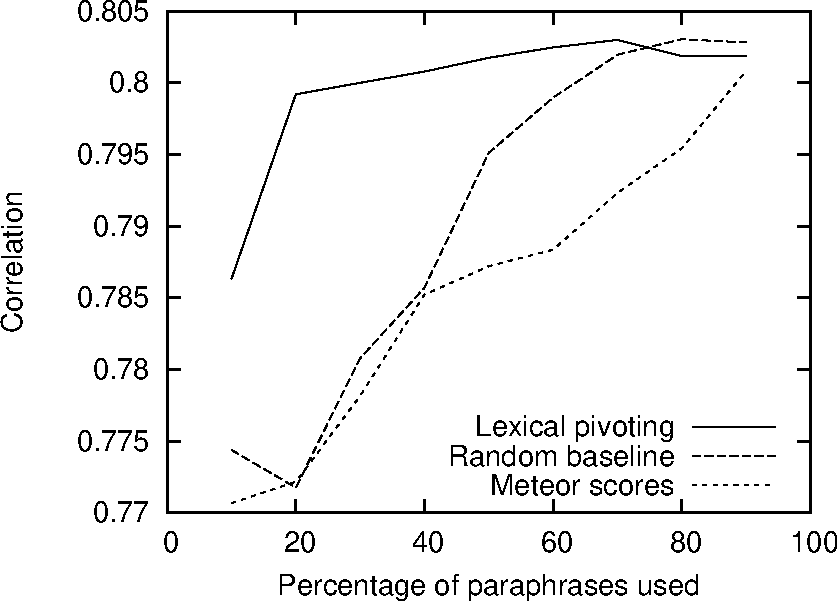
\includegraphics[scale=0.55]{filtering-lexical-cropped.pdf}
\caption{Comparison of automatic filtering techniques for~\emph{one-word} paraphrases on WMT12 data.}
\label{fig:filtering-lexical}
\end{center}
\end{figure}

\begin{figure}[ht]
\begin{center}
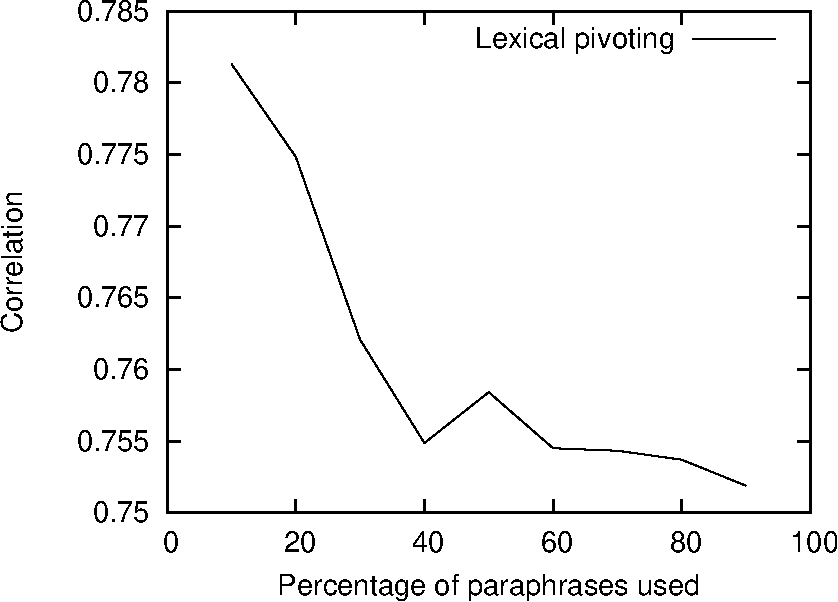
\includegraphics[scale=0.55]{filtering-mwe-cropped.pdf}
\caption{Automatic filtering of multi-word paraphrase for~the \textit{multi-word-first} scenario on WMT12 data.}
\label{fig:filtering-mwe}
\end{center}
\end{figure}


\Fref{fig:filtering-lexical} shows the performance of different filtering
techniques for one-word paraphrases. Relying on Meteor scores proves worse than
random selection. Using lexical pivoting, we can keep a high correlation even if we
throw away as much as 90\% of the paraphrases, however we do not improve 
(by~a~relevant margin) upon the baseline correlation of 0.802 achieved by
\emph{one-word-only} paraphrasing with the full paraphrase table.

We evaluate the best-performing technique also in the \textit{multi-word-first}
scenario where we use it for filtering multi-word paraphrases (see
\Fref{fig:filtering-mwe}). As we reduce the number of paraphrases, we observe a
considerable improvement of~correlation, however we never outperform
\textit{one-word-only} or \textit{one-word-first}. In this case, the filtering
simply mitigates the damage done by the multi-word paraphrases. We
cannot hope to achieve a higher score without a~more fine-grained grip on what
a~good multi-word paraphrase is.

\end{document}